\section{Database access models}

\begin{frame}
  \frametitle{Databases}
  \begin{example}[Typical relational database in a tax office]
  \begin{tabular}{l|l|l|l|l|l|l}
    ID & Name &  Salary & Deposits & Age & Postcode & Profession\\
    \hline
    1959060783 & Mike Pence & 150,000 & 1e6 & 60 & 1001 & Politician\\
    1946061408 & Donald Trump & 300,000 & -1e9 & 72 & 1001 & Rentier\\
    2100010101 & A. B. Student & 10,000 & 100,000 & 40 & 1001 & Time Traveller
  \end{tabular}
\end{example}

  \begin{block}{Database access}
    \begin{itemize}
    \item When owning the database: Direct look-up.
    \item When accessing a server etc: Query model.
    \end{itemize}
  \end{block}

  \begin{figure}[H]
    \centering
    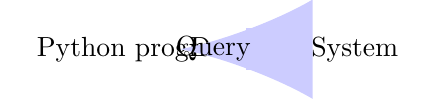
\begin{tikzpicture}
        \node at (0,0) (python) {Python program};
        \node at (2,0) (database) {Database System};
        \draw[->, >=latex, blue!20!white, line width=15pt]   (python) to node[black]{Query} (database) ;
      \end{tikzpicture}
    \label{fig:database-access}
    \caption{Database access model}
  \end{figure}

  
\end{frame}



%%% Local Variables:
%%% mode: latex
%%% TeX-master: "notes"
%%% End:
